\documentclass[conference]{IEEEtran}
\IEEEoverridecommandlockouts
% The preceding line is only needed to identify funding in the first footnote. If that is unneeded, please comment it out.
\usepackage{cite}
\usepackage{amsmath,amssymb,amsfonts}
\usepackage{algorithmic}
\usepackage{graphicx}
\usepackage{textcomp}
\usepackage{xcolor}
\usepackage{url}
\usepackage[colorlinks]{hyperref}
\usepackage{listings}
\usepackage{tikz}
\usepackage{tkz-euclide}
\usepackage{svg}

\usetikzlibrary{shapes,positioning,shapes.gates.logic}

\tikzset{ell/.style={circle,draw,minimum height=0.2cm,minimum width=0.2cm,inner sep=0.15cm}}
\tikzset{rec/.style={rectangle,draw,minimum height=0.5cm,minimum width=0.5cm,inner sep=0.2cm}}
\tikzset{trp/.style={trapezium,draw,trapezium left angle=120, trapezium right angle=120, minimum height=0.5cm}}


%New colors defined below
\definecolor{codegreen}{rgb}{0,0.6,0}
\definecolor{codegray}{rgb}{0.5,0.5,0.5}
\definecolor{codepurple}{rgb}{0.58,0,0.82}
\definecolor{backcolour}{rgb}{0.95,0.95,0.92}

%Code listing style named "mystyle"
\lstdefinestyle{mystyle}{
  backgroundcolor=\color{backcolour}, commentstyle=\color{codegreen},
  keywordstyle=\color{magenta},
  numberstyle=\tiny\color{codegray},
  stringstyle=\color{codepurple},
  basicstyle=\ttfamily\footnotesize,
  breakatwhitespace=false,         
  breaklines=true,                 
  captionpos=b,                    
  keepspaces=true,                 
  numbers=left,                    
  numbersep=5pt,                  
  showspaces=false,                
  showstringspaces=false,
  showtabs=false,                  
  tabsize=2
}

%"mystyle" code listing set
\lstset{style=mystyle}


\def\BibTeX{{\rm B\kern-.05em{\sc i\kern-.025em b}\kern-.08em
    T\kern-.1667em\lower.7ex\hbox{E}\kern-.125emX}}
\begin{document}

\title{A Performance Survey of \\Dynamic Branch Predictors
\thanks{}
}
\author{\IEEEauthorblockN{Daniela Trevina}
\IEEEauthorblockA{\textit{Department of EECS} \\
\textit{Texas A\&M University-Kingsville}\\
Kingsville, USA \\
daniela.trevino@students.tamuk.edu}
\and
\IEEEauthorblockN{Daniela Lopez}
\IEEEauthorblockA{\textit{Department of EECS} \\
\textit{Texas A\&M University-Kingsville}\\
Kingsville, USA \\
daniela.lopez@students.tamuk.edu}
\and
\IEEEauthorblockN{Mengxiang Jiang}
\IEEEauthorblockA{\textit{Department of EECS} \\
\textit{Texas A\&M University-Kingsville}\\
Kingsville, USA \\
mengxiang.jiang@students.tamuk.edu}
\and
\IEEEauthorblockN{Samah Allahyani}
\IEEEauthorblockA{\textit{Department of EECS} \\
\textit{Texas A\&M University-Kingsville}\\
Kingsville, USA \\
samah.allahyani@students.tamuk.edu}
\and
\IEEEauthorblockN{Ugochukwu Onyeakazi}
\IEEEauthorblockA{\textit{Department of EECS} \\
\textit{Texas A\&M University-Kingsville}\\
Kingsville, USA \\
ugochukwu.onyeakazi@students.tamuk.edu}
}

\maketitle

\begin{abstract}
    Due to the importance of branch prediction, running benchmark simulations is a good way to understand and evaluate different models. This paper discusses six different models (bimodal, gshare, perceptron, hashed perceptron, TAGE, LTAGE), and tests them using ChampSim on different SPEC benchmarks. The results are analyzed with further work suggested.
\end{abstract}

\section{Introduction} \label{sec:introduction}
Branch prediction is a crucial component in modern computer architecture to improve performance and energy efficiency. When executing a program, the processor encounters branches in the control flow, where it must decide which path to take based on a conditional statement. Incorrect branch predictions result in wasted computation cycles and negatively impact the overall performance of the system. To mitigate this issue, branch predictors are employed to predict the outcome of the conditional statements, and enable the processor to pre-fetch instructions from the predicted path, reducing the overhead of branching.

Here is a concrete example showcasing how even small improvements in branch prediction accuracy can result in huge performance improvments, from Onur Mutlu\cite{mutlu2023}. Assume the processor has 20 pipeline stages, with a 5-wide fetch. If 1 out of 5 instructions that are fetched is a branch (distributed uniformly), then here are time lengths to fetch 500 instructions and resulting instructions per cycle for different prediction accuracies:
\begin{enumerate}
    \item 60\%:\\
    100 + 20 * 40(branch penalty) = 900 cycles\\
    IPC = 500/900 = 0.555\\
    \item 90\%:\\
    100 + 20 * 10(branch penalty) = 300 cycles\\
    IPC = 500/300 = 1.666\\
    \item 99\%:\\
    100 + 20 * 1(branch penalty) = 120 cycles\\
    IPC = 500/120 = 4.166\\
    \item 100\%:\\
    100 cycles\\
    IPC = 500/100 = 5\\
\end{enumerate}
As one can see, going from 60\% accuracy to 90\% results in over 300\% performance improvement, and from 90\% to 99\% is similar.


Over the years, a variety of branch prediction models have been developed to improve the accuracy of predictions. These models range from static branch predictors that use heuristics to predict the outcome of branches, to more sophisticated dynamic branch predictors (note: all models tested in this paper are dynamic) that rely on past history to make predictions. Furthermore, the emergence of  machine learning and artificial intelligence has led to the development of more advanced branch prediction techniques for both static and dynamic branch predictors.

The aim of this paper is to explore some branch prediction models and compare their performances. We will examine the underlying principles of each model, the algorithms used to make predictions and their implementations in a simulated processor.

\section{Models} \label{sec:models}
In this section, we will cover the various branch predictor models used in the simulation.

\subsection{Bimodal Predictor} \label{ssec:bimodal}
This model was first proposed by James E. Smith as an improvement on the single-bit last-time predictor\cite{smith1981}. This is a local history predictor in the sense that the Program Counter (PC) is used to differentiate branches and their past outcomes. It stores two bits in the branch target buffer (BTB). These two bits encode a state machine with four states shown in Fig. 
\ref{fig:bimodal}. 
\begin{figure}
    \centering
    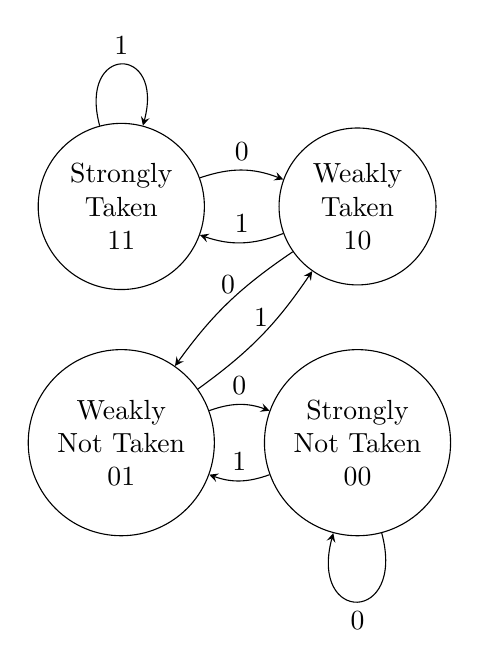
\begin{tikzpicture}[>=stealth]
		\node[ell,align=center] (st) at (0,3) {Strongly\\ Taken\\11};
        \node[ell,align=center] (wt) at (3,3) {Weakly\\ Taken\\10};
        \node[ell,align=center] (snt) at (3,0) {Strongly\\ Not Taken\\00};
        \node[ell,align=center] (wnt) at (0,0) {Weakly\\ Not Taken\\01};

        \draw [->] (st) to [loop above, looseness=5]node[]{1} (st);
        \draw [->] (st) to [bend left=20]node[above]{0} (wt);
        \draw [->] (wt) to [bend left=20]node[above]{1} (st);
        \draw [->] (wt) to [bend right=10]node[above]{0} (wnt);
        \draw [->] (wnt) to [bend right=10]node[above]{1} (wt);
        \draw [->] (wnt) to [bend left=20]node[above]{0} (snt);
        \draw [->] (snt) to [bend left=20]node[above]{1} (wnt);
        \draw [->] (snt) to [loop below, looseness=5]node[]{0} (snt);
    \end{tikzpicture}
    \caption{Bimodal Predictor}
	\label{fig:bimodal}
\end{figure}
The \textit{Strongly Taken} and \textit{Weakly Taken} states will predict \textit{taken} for the current branch, while the \textit{Strongly Not Taken} and \textit{Weakly Not Taken} states will predict \textit{not taken}. The actual result of the current branch causes the state transitions (1 for taken and 0 for not taken on the directed edges).

\subsection{Gshare Predictor} \label{ssec:gshare}
This model was first proposed by Scott McFarling as an improvement on the global history predictor\cite{mcfarling1993}. A normal global history predictor uses the single history from the Global History Register (GHR) to index into the Pattern History Table (PHT) in order to predict all branch outcomes regardless of the PC. Gshare XORs the PC with the GHR for indexing into the PHT, which adds some local history context information for the predictor to take into account.

\subsection{Perceptron Predictor} \label{ssec:perceptron}
This model is a single-layer version of an artificial neural network that can identify and classify patterns, first applied to branch prediction by Daniel A. Jimen\'ez and Calvin Lin\cite{jimenez2001dynamic}. In the model shown in Fig. \ref{fig:perceptron} are the input vector ($x$), the weight vector ($w$), and the output ($y$).
\begin{figure}
    \centering
    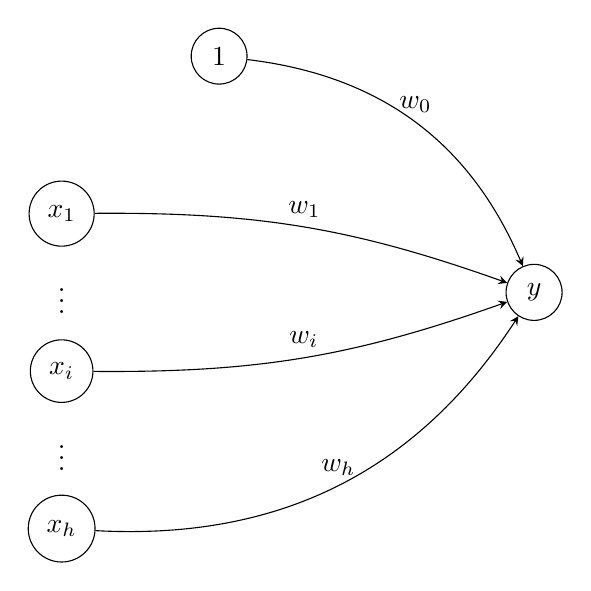
\begin{tikzpicture}[>=stealth]
		\node[ell] (x0) at (2,6) {$1$};
        \node[ell] (x1) at (0,4) {$x_1$};
        \node[] (x2) at (0,3) {\vdots};
        \node[ell] (xi) at (0,2) {$x_i$};
        \node[] (x3) at (0,1) {\vdots};
        \node[ell] (xh) at (0,0) {$x_h$};
        \node[ell] (y) at (6,3) {$y$};

        \draw [->] (x0) to [bend left]node[above]{$w_0$} (y);
		\draw [->] (x1) to [bend left=10]node[above]{$w_1$} (y);
		\draw [->] (xi) to [bend right=10]node[above]{$w_i$} (y);
		\draw [->] (xh) to [bend right]node[above]{$w_h$} (y);
    \end{tikzpicture}
    \caption{Perceptron Predictor}
	\label{fig:perceptron}
\end{figure}
The inputs correspond to values taken from the global history register, with the exception of $x_0$, the bias, always set to $1$. The output's sign determines the prediction. If the sign is negative, the branch is not taken, otherwise it is taken. Equation \eqref{eqn:1} shows the calculation of the output:
\begin{equation}
    y = w_o + \sum_{i=1}^{h}{x_iw_i}
    \label{eqn:1}
\end{equation}

The weights of the perceptron are trained using the algorithm below:
\begin{lstlisting}
if sgn(y) != t or abs(y) <= theta  then
    for i := 0 to n do
        w[i] := w[i] + t*x[i]
    end
end
\end{lstlisting}
$t$ is 1 if the branch is actually taken or -1 if not. $\theta$ is the threshold to determine when training should stop. $w_i$ is incremented if $t$ and $x_i$ agree, and decremented if they disagree.

\subsection{Hashed Perceptron (HP) Predictor} \label{ssec:hp}
This predictor is based off of the perceptron branch predictor from the previous section(\ref{ssec:perceptron}) but with a few important changes. The first change is instead of a single table for the weights, multiple independently indexed tables of perceptron weights are used, introduced by Jimen\'ez \cite{jimenez2003}.  The second is using the hash of the global history rather than just the global history for indexing in order to reduce the number of independent tables, contemporaneously by Seznec \cite{seznec2004}, Tarjan and Skadron\cite{skadron2004}, and Loh and Jimen\'ez\cite{loh2005reducing}.  The third is instead of using a fixed global history length, exponentially increasing global history lengths are used for indexing, by Seznec\cite{seznec2004gehl}\cite{seznec2005analysis}. This idea is actually one of the key parts of the TAGE predictor described in the next section(\ref{ssec:tage}). The last is to dynamically adjust the $\theta$ value for the training, also by Seznec\cite{seznec2004gehl}\cite{seznec2005analysis}.

\subsection{TAGE Predictor} \label{ssec:tage}
TAGE stands for TAgged GEometric history length branch predictor, and it was introduced by Andr\'e Seznec\cite{seznec2006case}. The first key idea, as mentioned earlier, is using exponentially increasing global history lengths for indexing into multiple tables, in this case PHTs while for the hashed perceptron it was the weights. The second is to intelligently allocate the PHT entries to different branches. Fig. \ref{fig:tage} shows a 3-component TAGE predictor, while the TAGE predictor evaluated in our simulations has 13 components.
\begin{figure}
    \centering
    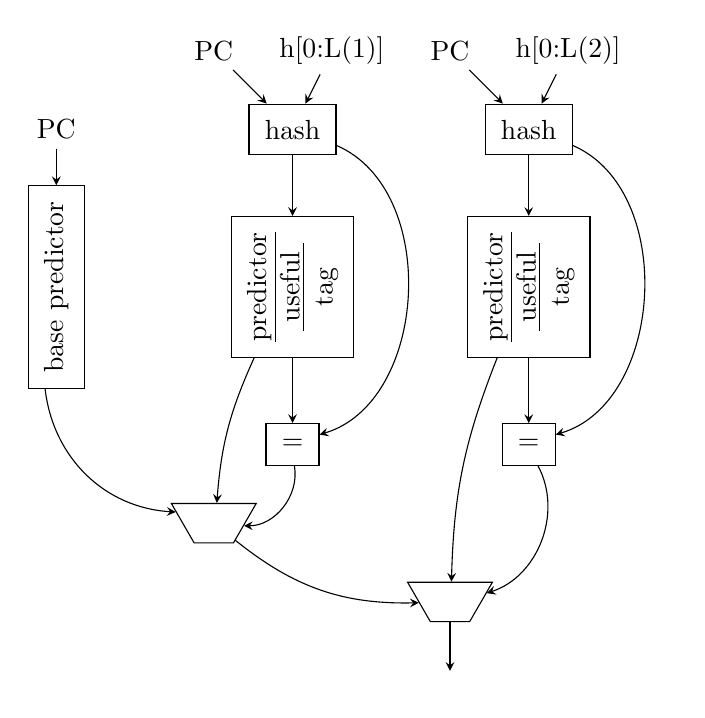
\begin{tikzpicture}[>=stealth]
		\node[] (pc0) at (0,11) {PC};
        \node[] (pc1) at (2,12) {PC};
        \node[] (pc2) at (5,12) {PC};
        \node[] (h1) at (3.5,12) {h[0:L(1)]};
        \node[] (h2) at (6.5,12) {h[0:L(2)]};
        \node[rec] (hash1) at (3, 11) {hash};
        \node[rec] (hash2) at (6, 11) {hash};
        \node[rec, rotate=90] (bp) at (0,9) {base predictor};
        \node[rec, rotate=90, align=center] (p1) at (3,9) {\underline{predictor}\\\underline{ useful }\\tag};
        \node[rec, rotate=90, align=center] (p2) at (6,9) {\underline{predictor}\\\underline{ useful }\\tag};
        \node[rec] (eq1) at (3,7) {=};
        \node[rec] (eq2) at (6,7) {=};
        \node[trp] (t0) at (2,6) {};
        \node[trp] (t1) at (5,5) {};
        \node[] (out) at (5,4) {};

        \draw [->] (pc0) to []node[]{} (bp);
        \draw [->] (bp) to [bend right=40]node[]{} (t0);
        \draw [->] (pc1) to []node[]{} (hash1);
        \draw [->] (h1) to []node[]{} (hash1);
        \draw [->] (hash1) to []node[]{} (p1);
        \draw [->] (hash1) to [bend left=70]node[]{} (eq1);
        \draw [->] (p1) to []node[]{} (eq1);
        \draw [->] (p1) to [bend right=10]node[]{} (t0);
        \draw [->] (eq1) to [bend left=50]node[]{} (t0);
        \draw [->] (pc2) to []node[]{} (hash2);
        \draw [->] (h2) to []node[]{} (hash2);
        \draw [->] (hash2) to []node[]{} (p2);
        \draw [->] (hash2) to [bend left=70]node[]{} (eq2);
        \draw [->] (p2) to []node[]{} (eq2);
        \draw [->] (p2) to [bend right=10]node[]{} (t1);
        \draw [->] (eq2) to [bend left=50]node[]{} (t1);
        \draw [->] (t0) to [bend right=20]node[]{} (t1);
        \draw [->] (t1) to []node[]{} (out);

    \end{tikzpicture}
    \caption{3-Component TAGE Predictor}
	\label{fig:tage}
\end{figure}

\subsection{LTAGE Predictor} \label{ssec:ltage}
This predictor is based off of the TAGE predictor from the previous section(\ref{ssec:tage}), but with the addition of a loop predictor. It was introduced by Seznec and won the 2nd Championship Branch Prediction competition\cite{seznec2004}. A loop predictor first predicts the limit on how many iterations the loop will execute. It keeps track of the number of times the loop as executed, and as long as this count is below the limit, it will predict taken. 

\section{Methodology} \label{sec:methodology}
The study conducts experiments using the ChampSim Simulator. Each predictor is implemented in the branch prediction unit of the simulator. The predictors are then tested on application benchmarks from Standard Performance Evaluation Corporation (SPEC) suite of benchmarks. The performance of each predictor is recorded and presented in the next section (\ref{sec:results}).

\subsection{Simulation Environment} \label{ssec:champsim}
ChampSim (Championship Simulator) uses a modular design and configurable structure to achieve a low barrier to entry into the field of microarchitectural simulation \cite{gober2022championship}.

ChampSim operates by analyzing program behavior through a process called tracing, which involves instrumenting and running the program offline to produce a summary of its activity. This trace can be saved and later used as a substitute for actual program execution during simulation. Although this method sacrifices some accuracy, particularly in terms of operating system interactions, it offers advantages in terms of reproducibility and simulation speed.

ChampSim consists of four types of modules: branch predictors, branch target buffers (BTBs), memory prefetchers, and cache replacement policies. Each cache and Translation Lookaside Buffer (TLB) also has its own prefetcher and replacement policy. These modules may be different across different cache and TLB levels, and even between cores. During configuration, ChampSim identifies all necessary modules and links their source as required. For our simulations, we only change which branch predictor to use in the configuration, leaving everything else in their default settings.

\subsection{Benchmarks} \label{ssec:benchmarks}
The Standard Performance Evaluation Corporation (SPEC) provides benchmark suites to evaluate performance and energy efficiency for computing systems. These benchmarks are designed to measure various aspects of computer performance, such as CPU speed, memory bandwidth, graphics performance, etc. This study makes use of four application benchmarks from the SPEC CPU benchmark suite. \textit{gcc} and \textit{perl} are used for testing integer arithmetic (SPECint). \textit{soplex} and \textit{povray} are used for testing floating point performance (SPECfp).

\subsection{Metrics} \label{ssec:metrics}
The performance of the branch predictors are evaluated using the following metrics:\\ 
\begin{enumerate}
    \item \textit{Instructions Per Cycle} (IPC): IPC is a measure of the average number of instructions executed in each clock cycle of the CPU. It is calculated by dividing the total number of instructions executed during a given time by the number of clock cycles used to execute those instructions. A higher IPC value indicates that the processor is able to execute more instructions per cycle, which translates into higher performance.
    $$
        IPC = \frac{\textit{Number of Instructions Committed}}{\textit{Simulation Time in Cycles}}
    $$
    \item \textit{Mispredictions Per Kilo Instructions} (MPKI): MPKI is a performance metric used to measure the accuracy of a processor's branch predictor. It represents the number of mispredicted branches per thousand instructions executed. It is calculated by dividing the total number of mispredicted branches by the total number of instructions executed, and then multiplying by 1000 to express the result in terms of mispredictions per thousand instructions. A lower MPKI value indicates better branch prediction accuracy and can lead to higher processor performance.
    $$
    MPKI = \frac{\textit{Number of Mispredictions}}{\textit{Number of Instructions Committed}} \times 100
    $$
    \item \textit{Accuracy}: Accuracy is the percentage of correct predictions made by the branch predictor. It is computed by dividing the number of correctly predicted branches by the total number of predicted branches and multiplying the result by 100. A higher accuracy value indicates that the branch predictor's predictions are closer to the actual branch outcomes, and thus the model's performance is more reliable.
    $$
        Accuracy = \frac{\textit{Number of Correct Predictions}}{\textit{Number of Branches Committed}} \times 100
    $$
\end{enumerate}
\section{Results and Discussion} \label{sec:results}
Each model was executed in the ChampSim simulator and the results for four benchmarks from the SPEC CPU benchmark suite were recorded. Table \ref{table:results} shows the performance of each model across the various benchmarks. In this section, we present a detailed discussion of the results obtained.
\begin{table*}[htbp]
    \caption{Performance Results}
    \begin{center}
    \begin{tabular}{|c|c|c|c|c|c|c|c|c|c|c|c|c|}
    \hline
    &\multicolumn{3}{|c|}{\textbf{Benchmark: gcc}}& \multicolumn{3}{|c|}{\textbf{Benchmark: perl}} & \multicolumn{3}{|c|}{\textbf{Benchmark: soplex}} & \multicolumn{3}{|c|}{\textbf{Benchmark: povray}}\\
    \hline
    \textbf{Predictors} & \textbf{IPC} & \textbf{MPKI} & \textbf{Accuracy} & \textbf{IPC}  & \textbf{MPKI} & \textbf{Accuracy} & \textbf{IPC} & \textbf{MPKI} & \textbf{Accuracy} & \textbf{IPC} & \textbf{MPKI} & \textbf{Accuracy} \\
    \hline
    \textbf{bimodal} & 2.18893 & 0.8116 & 0.995865 & 1.9339 & 3.97542 & 0.971272 & 0.287601 & 12.9765 & 0.928403 & 1.28419 & 10.5247 & 0.927332 \\
    \hline
    \textbf{gshare} & 2.20866 & 0.6419 & 0.996729 & 1.95874 & 4.05482 & 0.970698 & 0.287169 & 12.9904 & 0.928326 & 1.33658 & 8.4325 & 0.941778 \\
    \hline
    \textbf{hp} & 2.22541 & 0.51766 & 0.997362 & 2.02928 & 3.15328 & 0.977213 & 0.292012 & 10.9323 & 0.939681 & 1.41964 & 6.73906 & 0.95347 \\
    \hline
    \textbf{perceptron} & 2.21491 & 0.61248 & 0.996879 & 2.00043 & 3.3734 & 0.975622 & 0.288693 & 12.6598 & 0.93015 & 1.36391 & 7.75706 & 0.946441 \\
    \hline
    \textbf{TAGE} & 2.22633 & 0.5082 & 0.997411 & 2.03183 & 3.12708 & 0.977402 & 0.291466 & 11.2682 & 0.937828 & 1.42276 & 6.65282 & 0.954066 \\
    \hline
    \textbf{LTAGE} & 2.22616 & 0.50936 & 0.997405 & 2.03162 & 3.12894 & 0.977389 & 0.291411 & 11.2704 & 0.937816 & 1.4228 & 6.65236 & 0.954069 \\
    \hline
    \end{tabular}
    \label{table:results}
    \end{center}
\end{table*}

\begin{figure}[htbp]
    \centering
    \includegraphics[width=\columnwidth]{ipc\_int.png}
    \caption{IPC Results on Integer Benchmarks (all bar graphs made in \textit{python} using \textit{matplotlib})}
    \label{fig:ipc_int}
\end{figure}

\begin{figure}[htbp]
    \centering
    \includegraphics[width=\columnwidth]{mpki\_int.png}
    \caption{MPKI Results on Integer Benchmarks}
    \label{fig:mpki_int}
\end{figure}

\begin{figure}[htbp]
    \centering
    \includegraphics[width=\columnwidth]{accuracy\_int.png}
    \caption{Accuracy Results on Integer Benchmarks}
    \label{fig:accuracy_int}
\end{figure}
\pagebreak
Fig. \ref{fig:ipc_int}, Fig. \ref{fig:mpki_int} and Fig. \ref{fig:accuracy_int} show that for integer arithmetic testing, the HP Predictor, TAGE Predictor, and LTAGE Predictor showed the best performance in terms of IPC and accuracy for both gcc and perl benchmarks. Specifically, the TAGE Predictor displayed the highest IPC and accuracy for the gcc and perl benchmarks. It is worth noting that the Bimodal Predictor had the lowest IPC in gcc and perl. In terms of accuracy, the Gshare predictor had the lowest in the perl benchmark while the Bimodal had the lowest in gcc.

\begin{figure}[htbp]
    \centering
    \includegraphics[width=\columnwidth]{ipc\_fp.png}
    \caption{IPC Results on Floating Point Benchmarks}
    \label{fig:ipc_fp}
\end{figure}

\begin{figure}[htbp]
    \centering
    \includegraphics[width=\columnwidth]{mpki\_fp.png}
    \caption{MPKI Results on Floating Point Benchmarks}
    \label{fig:mpki_fp}
\end{figure}

\begin{figure}[htbp]
    \centering
    \includegraphics[width=\columnwidth]{accuracy\_fp.png}
    \caption{Accuracy Results on Floating Point Benchmarks}
    \label{fig:accuracy_fp}
\end{figure}

Fig. \ref{fig:ipc_fp}, Fig. \ref{fig:mpki_fp} and Fig. \ref{fig:accuracy_fp} show that the results for the floating point performance testing, the HP Predictor demonstrated the best performance in terms of IPC and accuracy in the soplex benchmark. Whereas in povray benchmark, the LTAGE demonstrated the best performance in both IPC and accuracy. TAGE Predictor and LTAGE Predictor showed very similar performance to each other, with only slight differences in their IPC and accuracy values. On the other hand, the Bimodal Predictor and Gshare Predictor exhibited the lowest performance in terms of IPC and accuracy for the soplex and povray benchmarks, respectively.

In terms of MPKI, the TAGE Predictor had the lowest MPKI values for two out four benchmarks, indicating fewer misses per thousand instructions compared to the other predictors. The Bimodal Predictor had the highest MPKI values for gcc and povray benchmarks, while the Gshare Predictor had the highest MPKI for the perl and soplex benchmark.

Overall, the HP Predictor, TAGE Predictor, and LTAGE Predictor consistently outperformed the other predictors in terms of IPC, accuracy, and MPKI across all four benchmarks. Among these three predictors, the TAGE Predictor showed the best performance for integer arithmetic performance testing while the LTAGE and HP showed the best performance for floating point performance testing. Note that the Bimodal Predictor and Gshare Predictor demonstrated the weakest performance in most cases, though they are much simpler in design and therefore cost less hardware.

\section{Conclusion} \label{sec:conclusion}
This paper explored some branch prediction techniques through implementation as well as a comparative study using simulation experiments on a range of benchmark suites. The experimental results demonstrate that the HP Predictor, TAGE Predictor, and LTAGE Predictor are the most effective branch prediction models, consistently outperforming the other predictors in terms of IPC, accuracy, and MPKI across different benchmarks. The commonality of these three predicators is the use of geometric global history lengths, suggesting the importance of this idea for branch predictions.

In the future we might incorporate more advanced branch prediction schemes such as TAGE-SC-L in our framework for comparison. Also, we could change the default configuration of the simulated processor to see what effects it would have. The code for this project is available at \url{https://github.com/kumj2028/ChampSim}.

\bibliographystyle{plain}
\bibliography{project}

\vspace{12pt}

\end{document}
